\documentclass[../DoAn.tex]{subfiles}
\begin{document}
\raggedbottom
Trong quá trình thực hiện đồ án, em đã suy nghĩ tới một số tính năng và mong muốn tích hợp vào hệ thống, cũng như gặp một số khó khăn nhất định và đã có giải pháp khắc phục. Vì vậy trong chương này em sẽ trình bày một số giải pháp và đóng góp của đồ án.

\section{Tính năng làm bài kiểm tra online}
\subsection{Đặt vấn đề}
Trên thực tế thì mỗi công ty lại có một quy trình tuyển dụng khác nhau. Trong số đó có những công ty lựa chọn hình thức kiểm tra kiến thức và kỹ năng online của ứng viên như là một phần để đánh giá ứng viên. Các hệ thống kiểm tra online hiện nay có rất nhiều và được xây dựng với các chức năng rất đa dạng, như là cung cấp nhiều hình thức câu hỏi, nhiều kiểu tạo đề thi, phân phối đề thi,... Và tất nhiên muốn sử dụng các hệ thống đó thì công ty sẽ cần trả phí trong khi có thể không sử dụng hết tất cả tính năng mà hệ thống đó cung cấp. Vì vậy em nảy ra một ý tưởng là tích hợp vào hệ thống hỗ trợ quản lý tuyển dụng và nhân sự \textbf{tính năng làm bài kiểm tra online}. Tính năng này nhằm thay thế các hệ thống kiểm tra online phức tạp, cung cấp các chức năng đủ dùng để đánh giá sơ bộ kiến thức và kỹ năng của ứng viên thông qua các bài kiểm tra. Trong quá trình xây dựng tính năng, có một số vấn đề phát sinh là: Làm sao để ứng viên làm được bài kiểm tra đó? Cách xử lý một số tình huống gian lận?

\subsection{Giải pháp}
Tính năng làm bài kiểm tra online có thể chia thành một số chức năng nhỏ hơn như sau:

\begin{itemize}
    \item Tạo chủ đề câu hỏi
    \item Tạo câu hỏi
    \item Tạo bài kiểm tra
    \item Chỉ định bài kiểm tra
    \item Làm và nộp bài kiểm tra
    \item Xem kết quả bài kiểm tra
\end{itemize}

Hệ thống sẽ có rất nhiều câu hỏi, để quản lý các câu hỏi này tốt hơn thì cách đơn giản nhất là chia vào các chủ đề khác nhau. Đó là lý do chức năng "Tạo chủ đề câu hỏi" ra đời. Từ đó để tạo một câu hỏi thì cần nội dung câu hỏi, loại câu hỏi, chủ đề, độ khó, các câu trả lời (nếu có), mã nguồn (nếu có). Hệ thống cung cấp ba loại câu hỏi là câu hỏi một lựa chọn, câu hỏi nhiều lựa chọn và câu hỏi tự luận. Nếu câu hỏi là một lựa chọn thì bắt buộc có một đáp án đúng, câu hỏi là nhiều lựa chọn thì có một hoặc nhiều đáp án đúng.

Để tạo một bài kiểm tra, hệ thống cung cấp hai chế độ là tạo thủ công và tạo ngẫu nhiên. Tạo bài kiểm tra thủ công có nghĩa là từ ngân hàng câu hỏi, người tạo sẽ lựa chọn một số lượng câu hỏi để thêm vào bài kiểm tra. Còn ở chế độ tạo ngẫu nhiên, hệ thống sẽ hiển thị các chủ đề đang có với số lượng câu hỏi ứng với từng độ khó. Như vậy, người tạo sẽ cần điền số lượng câu hỏi ứng với từng chủ đề và độ khó. Sau đó người tạo bấm nút tạo bài kiểm tra ngẫu nhiên thì hệ thống sẽ sinh ra một bài kiểm tra theo cấu hình mà người tạo đã chọn. Để tạo bài kiểm tra, người tạo cũng cần nhập hai thông tin bắt buộc là tiêu đề và thời gian làm bài.

Như đã trình bày ở phần vấn đề, làm sao để ứng viên làm được bài kiểm tra. Để giải quyết vấn đề này, hệ thống sẽ cung cấp tài khoản cho ứng viên, dùng tài khoản này ứng viên sẽ vào được hệ thống để làm bài kiểm tra. Cũng nhờ việc tạo tài khoản cho ứng viên bộ phận nhân sự chỉ cần chỉ định bài kiểm tra cho tài khoản đó là ứng viên có thể có quyền truy cập bài kiểm tra. Sau này nếu ứng viên trở thành nhân viên chính thức thì đây cũng chính là tài khoản của nhân viên. Còn nếu không, ứng viên vẫn có thể truy cập vào hệ thống bằng tài khoản này nếu như có động thái ứng tuyển những lần tiếp theo.

Sau khi ứng viên được chỉ định bài kiểm tra, ứng viên sẽ thấy bài kiểm tra đó ngay sau khi đăng nhập thành công. Ứng viên bấm vào bài kiểm tra để bắt đầu làm bài. Trước khi tính thời gian, hệ thống sẽ thông báo ứng viên chỉ được làm một lần duy nhất và không nên thoát bài kiểm tra trước khi nộp bài. Hệ thống cũng yêu cầu ứng viên bấm nút "Đồng ý làm bài" thì mới bắt đầu hiển thị bài kiểm tra và tính thời gian. Khi bài kiểm tra được hiển thị lên thì dựa vào thời gian làm bài (dữ liệu lấy từ phía backend) hệ thống sẽ hiển thị đồng hồ đếm ngược. Tuy nhiên ở đây sẽ có một số vấn đề. Đầu tiên, ứng viên có thể sẽ bấm nhầm vào nút tải lại trang và nếu vẫn lấy dữ liệu từ backend để đếm ngược thì sẽ thời gian sẽ bị tính lại từ đầu. Vì thế em sẽ lưu thời gian này vào bộ nhớ local và đồng bộ nó với thời gian đang hiển thị, cách này giúp đồng hồ đếm ngược luôn hiển thị đúng thời gian còn lại. Vấn đề tiếp theo là trong quá trình làm bài ứng viên cố tình đóng tab, như thế thời gian lưu ở local storage sẽ không thể được cập nhật. Chẳng hạn tại thời điểm đóng tab ứng viên còn 10 phút làm bài. Ứng viên đóng tab trong 5 phút rồi mở lại tab, thời gian còn lại vẫn sẽ là 10 phút. Để ngăn chặn vấn đề này, ngay khi ứng viên đồng ý làm bài kiểm tra, ở phía backend cũng sẽ đếm ngược thời gian làm bài, khi hết thời gian này tự động đóng bài kiểm tra lại (Hệ thống sẽ tính dư 30 giây để đề phòng các sự cố không mong muốn). Như thế ứng viên không thể gian lận về mặt thời gian được. Hệ thống cũng hỗ trợ nộp bài tự động, nếu ứng viên không gian lận về mặt thời gian, có làm ít nhất một câu và khi hết thời gian vẫn chưa nộp bài thì hệ thống sẽ tự động lưu lại bài thi. Các trường hợp gian lận về mặt thời gian hoặc là không làm câu hỏi nào thì hệ thống sẽ không ghi nhận kết quả. Tất nhiên trong quá trình làm bài kiểm tra thì ứng viên vẫn có thể gian lận bằng nhiều hình thức khác, còn hệ thống cố gắng giảm thiểu gian lận trong khả năng cho phép.

Sau khi ứng viên làm bài kiểm tra và kết quả được lưu lại, ứng viên sẽ thấy được kết quả sơ bộ (kết quả những câu hỏi trắc nghiệm). Phía bộ phận nhân sự cũng sẽ được thông báo về bài kiểm tra này và có thể xem chi tiết những câu trả lời của ứng viên. Chính những câu trả lời này là một nguồn căn cứ để đánh giá năng lực ứng viên. Hệ thống cũng hỗ trợ in bài kiểm tra thành file để lưu lại, vì những bài kiểm tra này có thể được sửa đổi để dùng lại cho những lần sau, vì vậy dữ liệu có thể sẽ không còn được chính xác.

\subsection{Kết quả}
Xây dựng một luồng hoàn chỉnh, bắt đầu từ việc bộ phận nhân sự tạo chủ đề câu hỏi và tạo các câu hỏi. Sau đó có thể tạo bài kiểm tra theo hai chế độ: Thủ công hoặc ngẫu nhiên. Tiếp đến là chỉ định bài kiểm tra cho tài khoản ứng viên. Ứng viên sau khi đăng nhập sẽ nhìn thấy bài kiểm tra được chỉ định. Khi bấm vào bài kiểm tra hệ thống yêu cầu xác nhận làm bài. Ứng viên bấm xác nhận làm bài, làm bài và nộp bài kiểm tra. Ứng viên có thể tự nộp bài trước khi hết thời gian, hoặc hệ thống sẽ tự động nộp bài của ứng viên. Ứng viên có thể xem kết quả bài làm sơ bộ và phía bộ phận nhân sự có thể xem chi tiết bài làm của ứng viên.

\section{Bài toán lưu trữ ảnh, file tài liệu}
\subsection{Đặt vấn đề}
Khi truy cập vào một ứng dụng web, người dùng rất dễ nhìn thấy các hình ảnh. Đó là ví dụ đơn giản nhất nói lên tầm quan trọng của việc quản lý các file cho ứng dụng. Các file đó có thể là hình ảnh, tài liệu, âm thanh,... Trong DATN thì các file được lưu trữ là các hình ảnh minh họa, avatar của các nhân viên, các file tài liệu của các chương trình đào tạo. Để quản lý các file này có nhiều cách, chẳng hạn như mã hóa dữ liệu rồi lưu vào cơ sở dữ liệu, hoặc là lưu trực tiếp ở máy chủ, hoặc tìm kiếm hỗ trợ của một bên thứ ba. Nhận định rằng nếu số lượng file là ít thì lưu trực tiếp ở máy chủ sẽ là lựa chọn tốt. Số lượng file nhiều có thể mã hóa để lưu vào cơ sở dữ liệu nhưng khi đó, cả lúc lưu và lúc lấy ra sử dụng đều mất công giải mã.

\subsection{Giải pháp}
Trong DATN sẽ sử dụng công cụ của bên thứ ba, đó là Cloudinary. Về cơ bản nền tảng này cho phép lưu trữ file ảnh và chỉnh sửa ảnh nếu cần thiết. Ngoài ra, Cloudinary cung cấp các tiện ích bổ sung (add-on), trong đó có tiện tích \textbf{Aspose Document Conversion}. Nhờ tiện ích này, có thể lưu trữ được các file không phải là ảnh lên Cloudinary. Sau đây sẽ là luồng hoạt động của ứng dụng kết hợp sử dụng Cloudinary:

\begin{figure}[H]
    \centering
    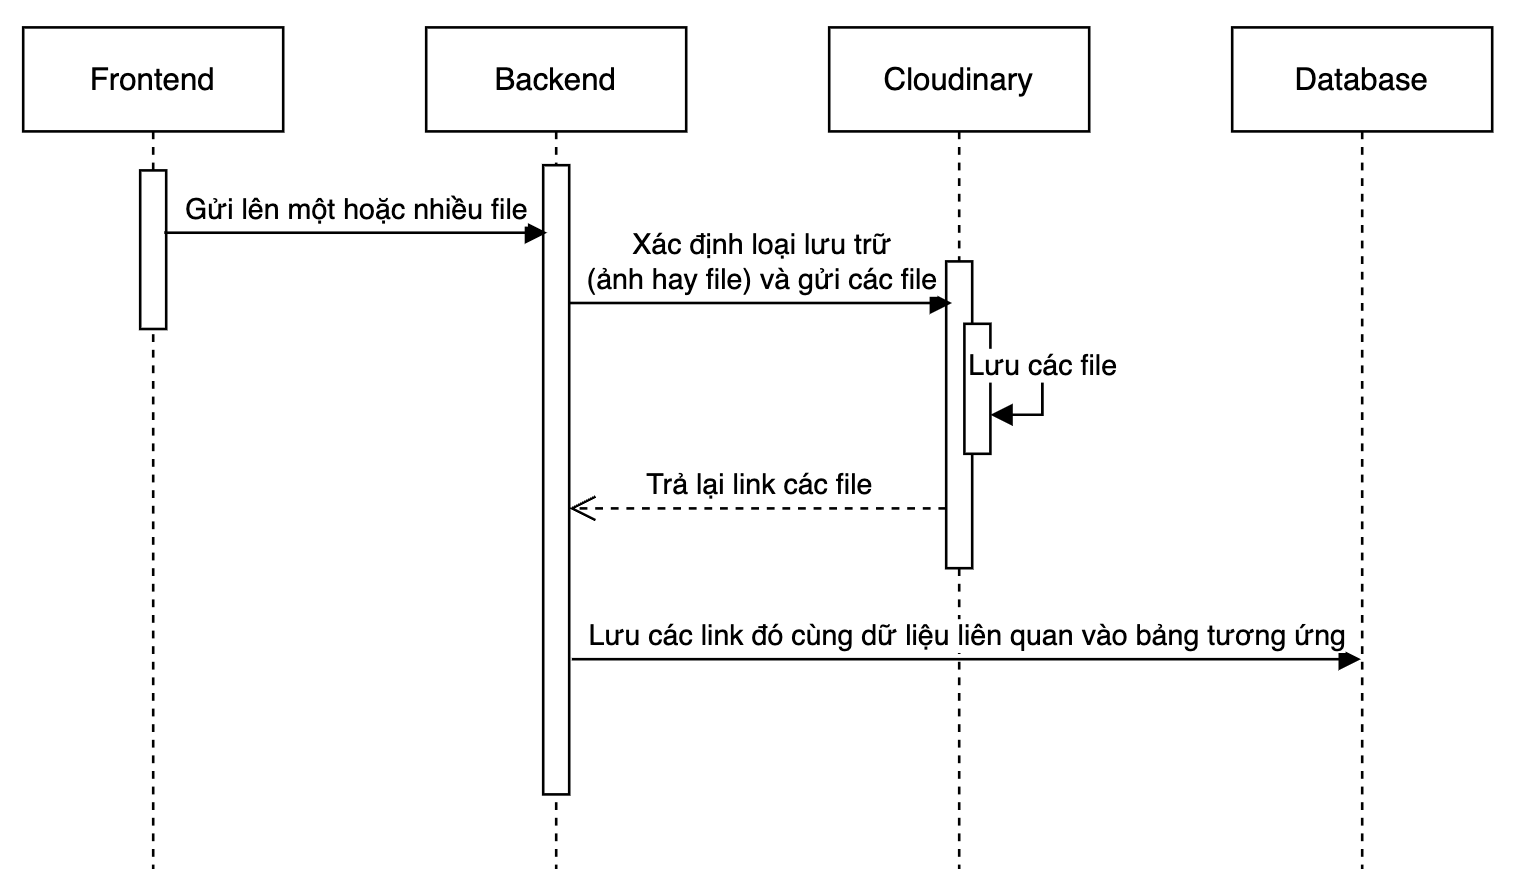
\includegraphics[width=0.9\linewidth]{Hinhve/LuongCloudinary.png}
    \caption{Luồng sử dụng Cloudinary}
\end{figure}

\subsection{Kết quả}
Ảnh và các file được lưu trữ trên Cloudinary sử dụng một cách bình thường.


\section{Bài toán quản lý thông báo}
\subsection{Đặt vấn đề}
Trong một ứng dụng có nhiều sự thay đổi thậm chí hằng ngày, hằng giờ thì việc có các thông báo cho những người sử dụng trong hệ thống là rất cần thiết. Chẳng hạn trong DATN này, mỗi khi một nhân viên tạo một request mới, hay một ứng viên làm xong bài kiểm tra mà ứng viên đó được chỉ định thì có thể thông báo cho bộ phận nhân sự, hoặc khi một chương trình đào tạo mới được công bố thì nên thông báo cho tất cả nhân viên trong công ty và còn rất nhiều tình huống khác nữa. Việc thông báo như vậy thực sự cần thiết để những thông tin quan trọng luôn được gửi tới mọi người một cách kịp thời, giúp mọi công việc trong công ty trơn tru, tránh được các nhầm lẫn hay bỏ lỡ thông tin không đáng có. Đặc biệt, những thông báo này nên theo thời gian thực, nghĩa là khi có một sự kiện quan trọng xảy ra thì nên thông báo ngay lúc ấy. Để làm được điều đó cũng có nhiều cách làm như là thông báo qua email, hoặc sử dụng công nghệ socket, hoặc sử dụng công cụ của các bên thứ ba. Nếu tự dùng socket để xây dựng chức năng thông báo này sẽ khó khăn trong việc quản lý trạng thái ứng dụng nếu số lượng kênh nhiều và số kết nối socket lớn.

\subsection{Giải pháp}
Trong DATN có xây dựng chức năng gửi email tự động. Tuy nhiên trong việc quản lý các thông báo như trên thì em hướng tới việc hiển thị thông báo ngay trên chính giao diện ứng dụng. Sử dụng socket có thể giúp làm được điều này, tuy nhiên như đã nói, việc quản lý các kết nối có thể sẽ gặp khó khăn. Vì thế DATN tích hợp thêm một công cụ là Novu\cite{Novu}. Novu giúp lưu trữ tất cả các thông báo của ứng dụng, hỗ trợ tạo các loại thông báo, tùy chỉnh nội dung cho từng loại thông báo. Novu cũng cho phép tạo các chủ đề (topic) và thêm người đăng ký chủ đề cho topic đó. Bằng cách này, ứng dụng có thể gửi thông báo cho một nhóm người cụ thể. Chẳng hạn, thông báo khi nhân viên tạo mới một request chỉ gửi cho người quản lý khối của nhân viên đó và các quản trị viên mà thôi. Hỗ trợ làm việc với Novu là hai thư viện \textbf{@novu/node} hỗ trợ phía backend và \textbf{@novu/notification-center} hỗ trợ phía frontend. 

\subsection{Kết quả}
Hiển thị danh sách các thông báo bao gồm cả những thông báo đã/chưa đọc. Người dùng click vào một thông báo thì thông báo ấy sẽ được đánh dấu là đã đọc. Người dùng cũng có thể đánh dấu trạng thái đã đọc cho tất cả các thông báo.


\section{Giao tiếp thông qua kênh chat}
\subsection{Đặt vấn đề}
Thông thường, ứng viên nếu muốn trao đổi với phía nhân sự của công ty thì có nhiều cách như trao đổi qua email, số điện thoại hoặc qua các mạng xã hội. Với mục đích tạo thêm một kênh liên hệ cho các ứng viên, DATN mong muốn tích hợp một module mà ở đó ứng viên khi vào trang chủ của công ty có thể chat trực tiếp với bộ phận
nhân sự.

\subsection{Giải pháp}
Trong DATN này sử dụng Chatwoot\cite{Chatwoot} là một nền tảng cho phép tích hợp tính năng chat vào ứng dụng web/app. Chatwoot cung cấp dashboard quản lý tất cả các phiên trao đổi. Người dùng khi truy cập vào ứng dụng web/app sẽ thấy biểu tượng chat, nhấn vào sẽ hiện ra cửa sổ chat và từ đó người dùng bắt đầu phiên trao đổi của mình. Chatwoot cũng hỗ trợ thu thập thông tin người dùng. Chẳng hạn trước khi người dùng bắt đầu trao đổi, có thể hiển thị một form (có thể tùy chỉnh form này theo nhu cầu) và yêu cầu người dùng gửi một số thông tin cơ bản như tên, số điện thoại, email,... Các thông tin này là hữu ích để bộ phận nhân sự nắm được những ai đang quan tâm đến việc làm của công ty và những công việc nào đang được quan tâm nhất. Ngoài ra, Chatwoot cũng cho phép kết nối với các bot nhằm giúp thay thế con người khi mà bộ phận nhân sự chưa kịp trả lời ứng viên. Tuy nhiên trong phạm vi của DATN này sẽ chưa tích hợp các bots đó.

\subsection{Kết quả}
Ứng viên có thể trao đổi với bộ phận nhân sự qua kênh chat này. Kênh chat cũng hỗ trợ thu thập thông tin ứng viên thông qua form trước khi bắt đầu phiên trao đổi.

\section{Bài toán phân quyền cho ứng dụng}
\subsection{Đặt vấn đề}
Trong một ứng dụng quản lý nói chung luôn có nhu cầu bảo mật thông tin. Một trong những bài toán cụ thể là là làm sao để mỗi người trong hệ thống ấy chỉ được truy cập vào tài nguyên đúng với vai trò của mình. Chẳng hạn quản trị viên có thể xem được mọi thông tin, điều chỉnh được mọi loại dữ liệu nhưng một người dùng bình thường sẽ chỉ xem được các thông tin công cộng hoặc là những thông tin liên quan đến bản thân mình thôi. Đó chính là bài toán phân quyền. Phân quyền ở đây phải được thực hiện trên cả frontend lẫn backend. Phía frontend với mỗi người, mỗi quyền hạn khác nhau lại hiển thị những chức năng khác nhau. Với mỗi yêu cầu gửi đến backend, backend sẽ kiểm duyệt người gửi có được phép truy cập vào tài nguyên tương ứng hay không. Ở trong DATN này, việc phân quyền rất quan trọng bởi ứng dụng có tới sáu tác nhân. Cần làm sao để mỗi tác nhân ấy chỉ được sử dụng những tính năng trong quyền hạn của mình.

\subsection{Giải pháp}
Hệ thống có những chức năng không giới hạn quyền truy cập và những chức năng giới hạn quyền truy cập. Với những chức năng có giới hạn đó, người truy cập cần có một tài khoản và tài khoản đó có thể là của ứng viên hoặc là của nhân viên. Đối với tài khoản nhân viên sẽ được kết nối với một hồ sơ nhân viên, trong hồ sơ ấy sẽ có thông tin mô tả vai trò của nhân viên trong hệ thống (nhân viên bình thường, quản lý khối, quản trị viên hay quản trị viên tối cao), còn lại là các tài khoản ứng viên. Vì thế về mặt giao diện, ta hoàn toàn phân biệt được tài khoản đó có quyền hạn gì trong hệ thống, từ đó hiển thị những chức năng tương ứng. Tuy nhiên phần quan trọng hơn cả là ở phía backend. Bởi lẽ người ta hoàn toàn có thể gửi các yêu cầu tới backend mà không gửi từ giao diện. Để giải quyết bài toán này, phía backend sẽ cấu hình các tài nguyên theo định dạng:

\begin{verbatim}
   role = {
     route_1: [method_1],
     route_2: [method_1, method_2,...],
     ...
   }
\end{verbatim}

Trong đó role là quyền hạn của tài khoản, route\_x là đường dẫn để lấy tài nguyên, còn method\_x là phương thức HTTP của yêu cầu gửi đến hệ thống (GET, POST, PUT, PATCH,...). Vậy làm sao để lấy được role? Mỗi khi người dùng đăng nhập vào hệ thống, hệ thống sẽ cung cấp một mã token như là chìa khóa truy cập vào các tài nguyên. Token này sẽ chứa được nhiều thông tin trong đó có thông tin role của người dùng. Có thông tin role, route và method của yêu cầu gửi đến ta sẽ so sánh với cấu hình ở trên xem người dùng này có được phép truy cập tài nguyên không, từ đó gửi trả kết quả phù hợp. Có thể tóm tắt thành một luồng hoạt động như sau:

\begin{figure}[H]
    \centering
    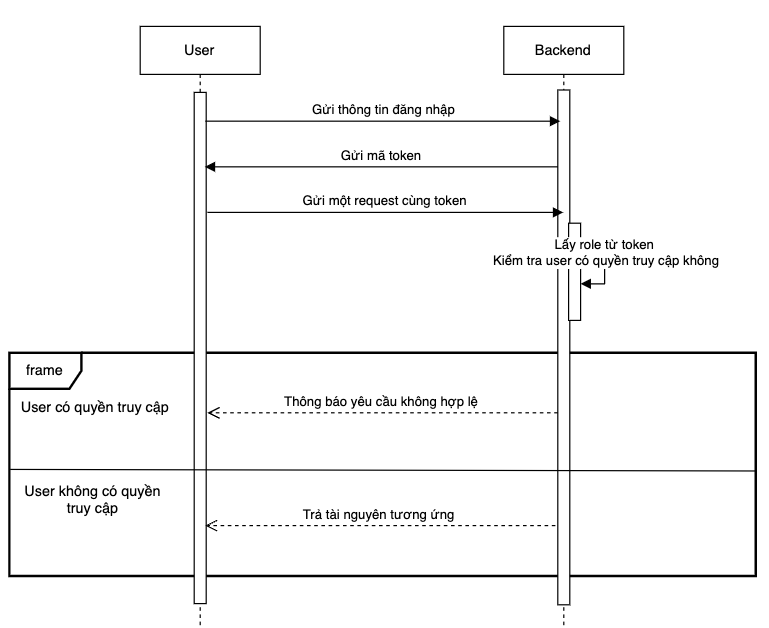
\includegraphics[width=0.9\linewidth]{Hinhve/PhanQuyenNguoiDung.png}
    \caption{Luồng phân quyền người dùng}
\end{figure}

\subsection{Kết quả}
Ứng dụng được phân quyền chính xác đối với quyền hạn của mỗi tài khoản.

\end{document}